\documentclass{article}
\usepackage[margin=1in]{geometry}
\usepackage{enumitem}
\usepackage{setspace}
\usepackage{amsmath}
\usepackage{amssymb}
\usepackage{physics}
\usepackage{graphicx}

\title{Math 151B Homework 5}
\date{9/7/2020}
\author{Jiaping Zeng}

\begin{document}
\setstretch{1.75}
\maketitle

\begin{itemize}
    \item [Q1] Euler's method: $w_{i+1}=w_i+hf(t_i,w_i)=w_i+h\lambda w_i=(1+h\lambda)w_i$, then $R=\{h\lambda\in C\mid\abs{1+h\lambda}<1\}$\\Midpoint method: $w_{i+1}=w_i+hf(t_i+\frac{h}{2},w_i+\frac{h}{2}f(t_i,w_i))=w_i+h\lambda(w_i+\frac{h\lambda}{2}w_i)=(1+h\lambda+\frac{(h\lambda)^2}{2})w_i$, then $R=\{h\lambda\in C\mid\abs{1+h\lambda+\frac{(h\lambda)^2}{2}}<1\}$\\Let $z=h\lambda=a+ib$, then we have $\abs{1+a+ib}<1\implies\sqrt{(1+a)^2+b^2}<1$ for Euler's method and $\abs{1+a+ib+\frac{(a+ib)^2}{2}}<1\implies\sqrt{(1+a+\frac{a^2-b^2}{2})^2+(b+ab)^2}<1$.
          \begin{center}
              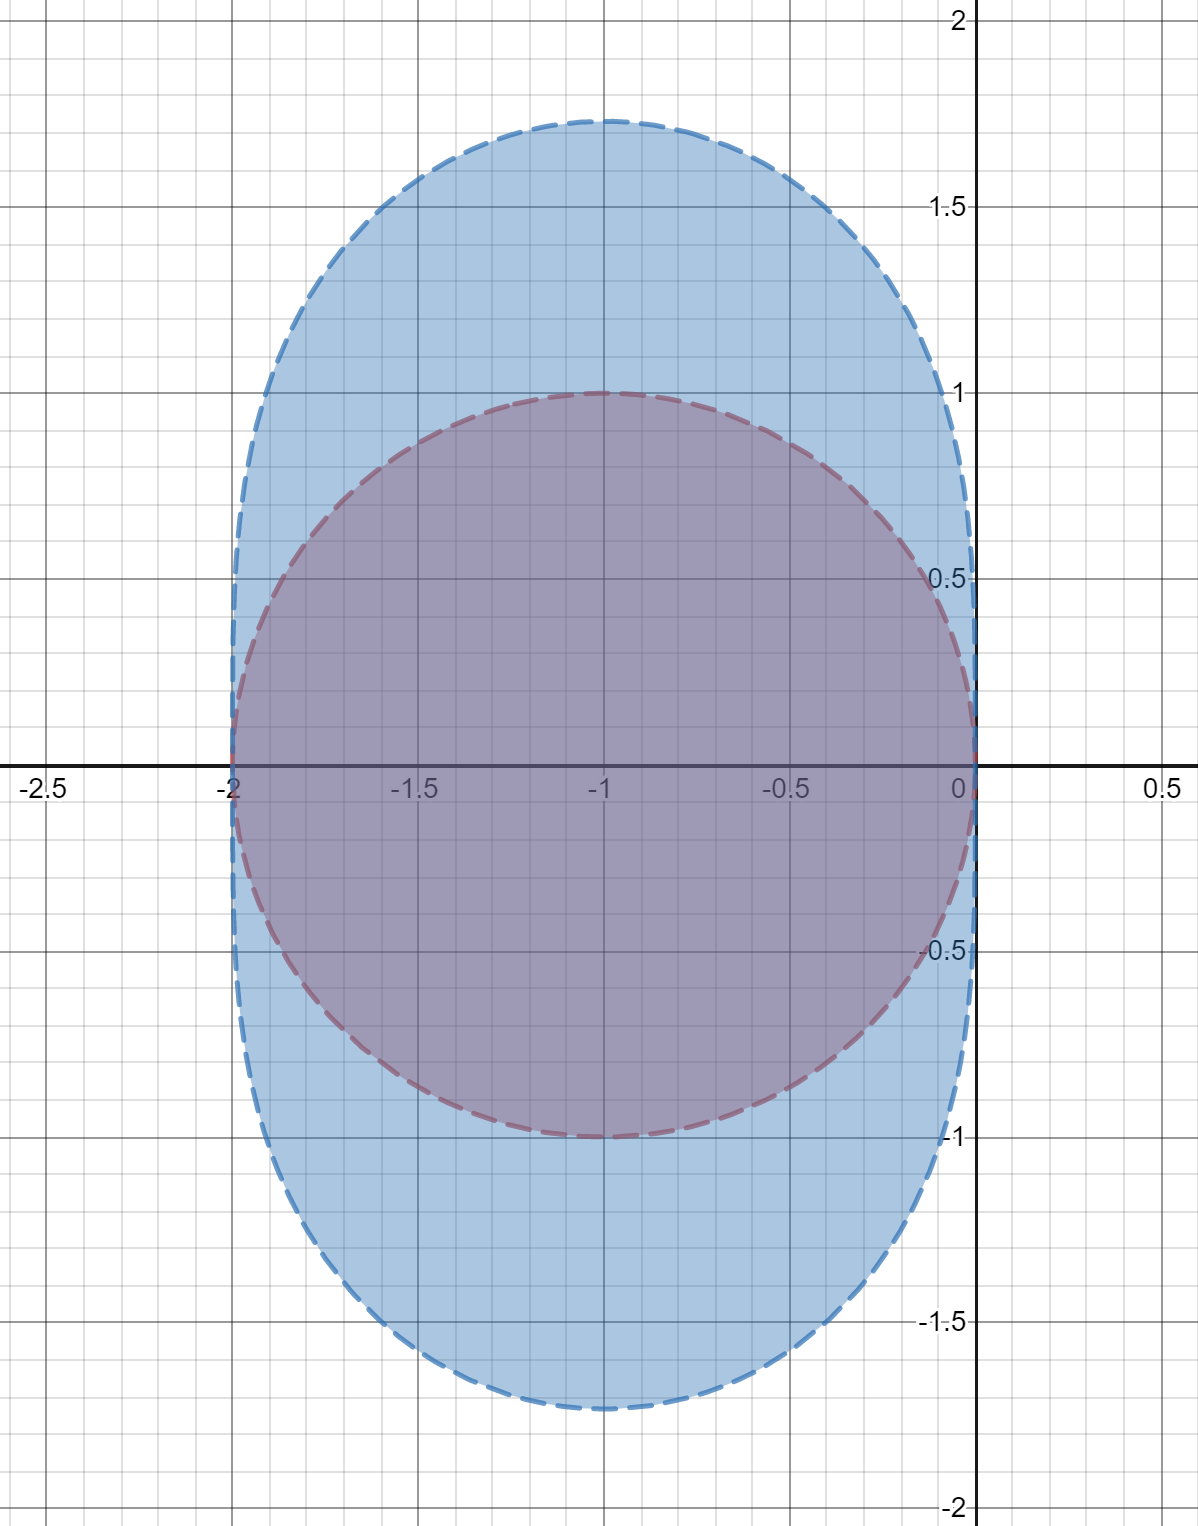
\includegraphics[width=4in]{graph.png}
          \end{center}
    \item [Q2]
          \begin{itemize}
              \item [(a)] For $h=\frac{\pi}{4}$, we have\\
                    \begin{tabular}{|c|c|c|}
                        \hline
                        $x_i$           & $w_i$         & error               \\
                        \hline
                        $\frac{\pi}{4}$ & $-0.28245222$ & $3.91\cdot 10^{-4}$ \\
                        \hline
                    \end{tabular}
              \item [(b)] For $h=\frac{\pi}{8}$, we have\\
                    \begin{tabular}{|c|c|c|}
                        \hline
                        $x_i$            & $w_i$         & error               \\
                        \hline
                        $\frac{\pi}{8}$  & $-0.31541496$ & $1.72\cdot 10^{-5}$ \\
                        \hline
                        $\frac{\pi}{4}$  & $-0.28285070$ & $7.99\cdot 10^{-6}$ \\
                        \hline
                        $\frac{3\pi}{8}$ & $-0.20718437$ & $8.61\cdot 10^{-6}$ \\
                        \hline
                    \end{tabular}
          \end{itemize}
    \item [Q3] Since $y''=p(x)y'+q(x)y\implies y''-p(x)y'-q(x)=0$, $y\equiv 0$ is a solution. Then by Corollary 11.2, the BVP $y''=p(x)y'+q(x)y$, for $a\leq x\leq b$, with $y(a)=0$ and $y(b)=0$ has a unique solution, i.e. $y\equiv 0$ is the only solution. Therefore $y_2\equiv 0$.
    \item [Q4] Using central-finite-difference we have $y''-4y=-4x\implies\frac{w_{i+1}-2w_i+w_{i-1}}{h^2}-4w_i=\frac{-4i}{N}$. Now for the boundaries, we can first use Taylor expansion as follows: $y(x+h)=y(x)+hy'(x)+\frac{h^2}{2}y''(x)+O(h^3)\implies y'(x)=\frac{y(x+h)-y(x)}{h}-\frac{h}{2}y''(x)$, then $w_i'=\frac{w_{i+1}-w_i}{h}-\frac{h}{2}w_i''=\frac{w_{i+1}-w_i}{h}-\frac{h}{2}w_i''=\frac{w_{i+1}-w_i}{h}-\frac{h}{2}(\frac{w_2-2w_1+w_0}{2h})=\frac{-3w_0+4w_1-w_2}{2h}$.\\
    So for $i=0$ we have $\frac{-3w_0+4w_1-w_2}{2h}=0\implies \frac{-3}{2h}w_0+\frac{2}{h}w_1-\frac{1}{2h}w_2=0$,\\
    for $i=1,\ldots,(N-1)$ we have $\frac{w_{i+1}-2w_i+w_{i-1}}{h^2}-4w_i=\frac{-4i}{N}\implies \frac{1}{h^2}w_{i-1}+\frac{-4h^2-2}{h^2}w_i+\frac{1}{h^2}w_{i+1}=-\frac{4i}{N}$,\\
    for $i=N$ we have $w_N=y(1)=1$. Then we can set up the matrix as follows: \[\begin{pmatrix}
        -\frac{3}{2h}&\frac{2}{h}&-\frac{1}{2h}&0&\ldots&\ldots&0\\
        \frac{1}{h^2}&\frac{-4h^2-2}{h^2}&\frac{1}{h^2}&0&\ldots&\ldots&0\\
        0&\frac{1}{h^2}&\frac{-4h^2-2}{h^2}&\frac{1}{h^2}&0&\ldots&0\\
        \ddots&\ddots&\ddots&\ddots&\ddots&\ddots&\ddots\\
        \ddots&\ddots&\ddots&\ddots&\ddots&\ddots&\ddots\\
        0&\ldots&\ldots&0&\frac{1}{h^2}&\frac{-4h^2-2}{h^2}&\frac{1}{h^2}\\
        0&\ldots&\ldots&\ldots&\ldots&0&1
    \end{pmatrix}\begin{pmatrix}
        w_0\\w_1\\w_2\\\vdots\\\vdots\\w_{N-1}\\w_N
    \end{pmatrix}=\begin{pmatrix}
        0\\-\frac{4}{N}\\-\frac{8}{N}\\\vdots\\\vdots\\-\frac{4(N-1)}{N}\\1
    \end{pmatrix}\]
\end{itemize}
\end{document}